
\subsection{Hamming}

\newpage
\subsection{Perceptron}
\textbf{Experimento 1}
\textbf{Experimento 2}
\subsection{ADALINE}
Los experimentos en ADALINE consistieron se dividieron en dos partes, la primera para pruebas que involucraran bias en donde se introdujo un archivo con el conjunto de entrenamiento al igual que en el perceptron, y por otro lado para la parte en la que no se utilizo el bias sólo se resolvió el problema del codificador en el cual el usuario indica el tamaño del codificador y la red comienza a trabajar como lo haría comúnmente.

Ambos tipos de experimentos incluyen la graficación de la evolución del error por iteración y de los valores de pesos y bias, además de que los valores finales son almacenados en un archivo llamado \emph{resultado\_hora\_fecha.txt}
\begin{figure}[H]
    \begin{center}
        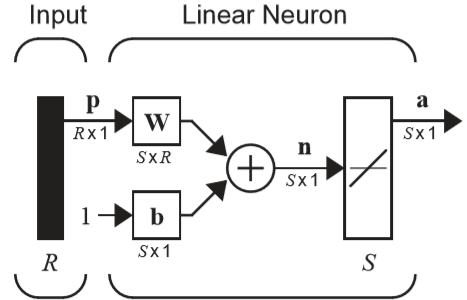
\includegraphics[width=9cm]{img/adaline/arquitectura.png}
        \caption{Arquitectura de la red ADALINE con bias. \cite{libro1}}
        \label{fig:adaline-diagrama2}
    \end{center}
\end{figure}
\subsubsection{Con bias}
\textbf{Experimento 1}
El conjunto de entrenamiento que se utilizo en este caso fue.
\[ \left\lbrace \boldsymbol{p_1} = \left[\begin{array}{c} 0\\ 0\end{array}\right], t_1 = -1  \right\rbrace, \left\lbrace \boldsymbol{p_2} = \left[\begin{array}{c} 0\\ 1\end{array}\right], t_2 = -1  \right\rbrace, \left\lbrace \boldsymbol{p_3} = \left[\begin{array}{c} 1\\ 0\end{array}\right], t_3 = -1  \right\rbrace, \left\lbrace \boldsymbol{p_4} = \left[\begin{array}{c} 1\\ 1\end{array}\right], t_4 = 1  \right\rbrace  \]
El cual corresponde a una compuerta AND de dos entradas. Esto provoco que los valores asociados a nuestra arquitectura de la figura \ref{fig:adaline-diagrama2} fueran los siguientes.
\begin{align*}
S=1 && R=2
\end{align*}
Además los valores asociados a $\boldsymbol{W}$ y $\boldsymbol{b}$ fueron números aleatorios pequeños. De igual forma se ingresan los valores para el factores de aprendizaje, número máximo de iteraciones y el mínimo error permitido, $\alpha=.03$, $it_{max}=100$, $e_{it}=.1$ respectivamente.
\begin{figure}[H]
    \begin{center}
        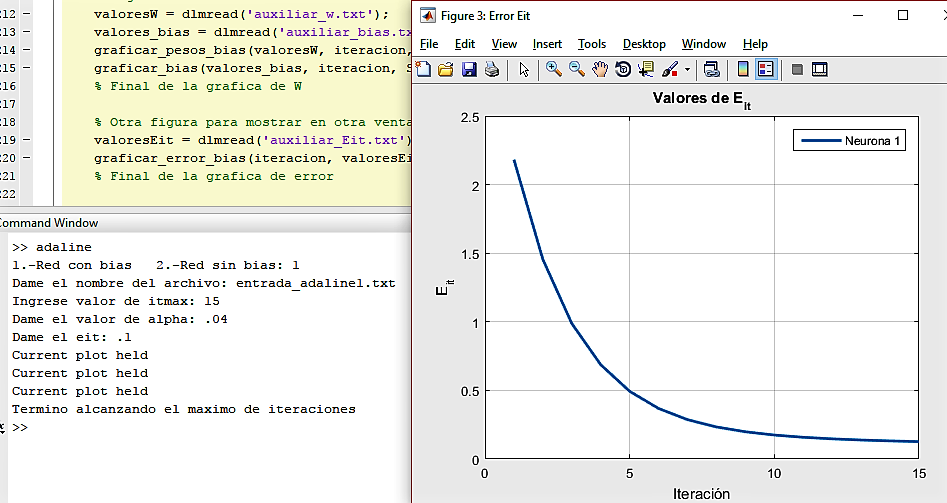
\includegraphics[width=16cm]{img/adaline1/error.png}
        \caption{Prueba 1 de ADALINE con bias.}
        \label{fig:adaline1error}
    \end{center}
\end{figure}
En la figura \ref{fig:adaline1error} se puede observar que la red llego a un resultado en la iteración 25 debido al criterio de error menor al permitido por iteración como se ve reflejado en la gráfica correspondiente, dando como resultado los siguientes valores para los pesos y bias.
\begin{align*}
\boldsymbol{W} = \left[\begin{array}{cc}0.5744 & 0.5956\end{array}\right] && \boldsymbol{b} = -0.9391
\end{align*}
Estos valores son almacenados en su respectivo archivo \emph{resultado\_hora\_fecha.txt}, en la figura \ref{fig:adaline1pesos} se puede observar su evolución a lo largo de las 25 iteraciones.
\begin{figure}[H]
    \begin{center}
        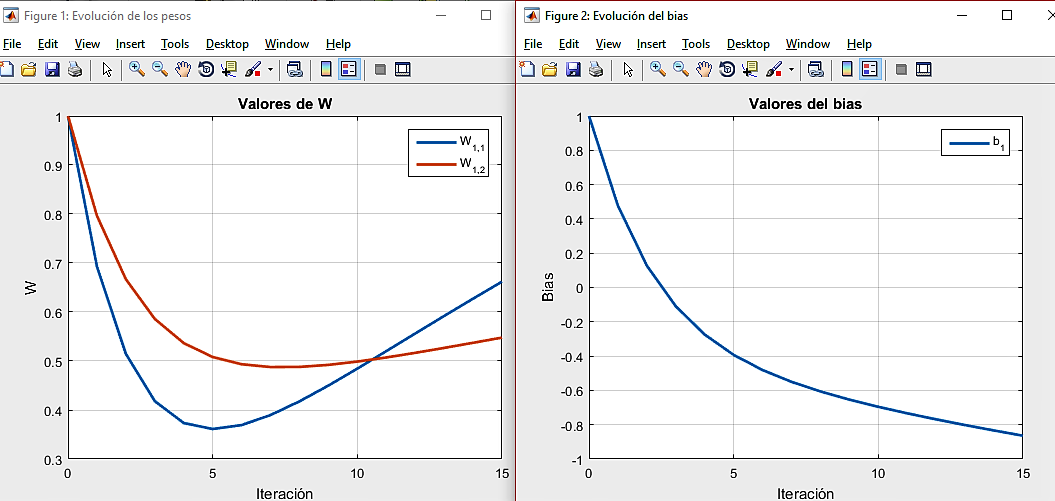
\includegraphics[width=16cm]{img/adaline1/pesosbias.png}
        \caption{Pesos y bias en esta prueba.}
        \label{fig:adaline1pesos}
    \end{center}
\end{figure}
\textbf{Experimento 2}
El conjunto de entrenamiento que se utilizo para entrenar a la red fue.
\[ \left\lbrace \boldsymbol{p_1} = \left[\begin{array}{c} 1\\ 1\end{array}\right], \boldsymbol{t_1} = \left[\begin{array}{c} -1\\ -1\end{array}\right]  \right\rbrace, \left\lbrace \boldsymbol{p_2} = \left[\begin{array}{c} 2\\ 0\end{array}\right], \boldsymbol{t_2} = \left[\begin{array}{c} -1\\ -1\end{array}\right]  \right\rbrace, \left\lbrace \boldsymbol{p_3} = \left[\begin{array}{c} -1\\ -1\end{array}\right], \boldsymbol{t_3} = \left[\begin{array}{c} -1\\ 1\end{array}\right]  \right\rbrace,\]

\[ \left\lbrace \boldsymbol{p_4} = \left[\begin{array}{c} 0\\ -1\end{array}\right], \boldsymbol{t_4} = \left[\begin{array}{c} -1\\ 1\end{array}\right]  \right\rbrace, \left\lbrace \boldsymbol{p_5} = \left[\begin{array}{c} -2\\ 0\end{array}\right],\boldsymbol{t_5} = \left[\begin{array}{c} 1\\ -1\end{array}\right]  \right\rbrace, \left\lbrace \boldsymbol{p_6} = \left[\begin{array}{c} -1\\ 1\end{array}\right], \boldsymbol{t_6} = \left[\begin{array}{c} 1\\ -1\end{array}\right]  \right\rbrace,\]

\[ \left\lbrace \boldsymbol{p_7} = \left[\begin{array}{c} 0\\ 2\end{array}\right], \boldsymbol{t_7} = \left[\begin{array}{c} 1\\ 1\end{array}\right]  \right\rbrace, \left\lbrace \boldsymbol{p_8} = \left[\begin{array}{c} 1\\ 2\end{array}\right], \boldsymbol{t_8} = \left[\begin{array}{c} 1\\ 1\end{array}\right]  \right\rbrace\]
Es por estos valores que las dimensiones de la red mostrada en la figura \ref{fig:adaline-diagrama2} quedan definidas de la siguiente forma.
\begin{align*}
S = 2 && R = 2
\end{align*}
Lo cual crea una matriz de pesos de $2x2$ y una matriz de bias de $2x1$ con valores aleatorios pequeños, mientras que los valores de iteración máxima, factor de aprendizaje y error permitido son de nueva cuenta introducidos manualmente de la forma $it_{max}=20$, $\alpha=0.04$,  $e_{it}=0.1$ respectivamente (véase figura \ref{fig:adaline2error}).
\begin{figure}[H]
    \begin{center}
        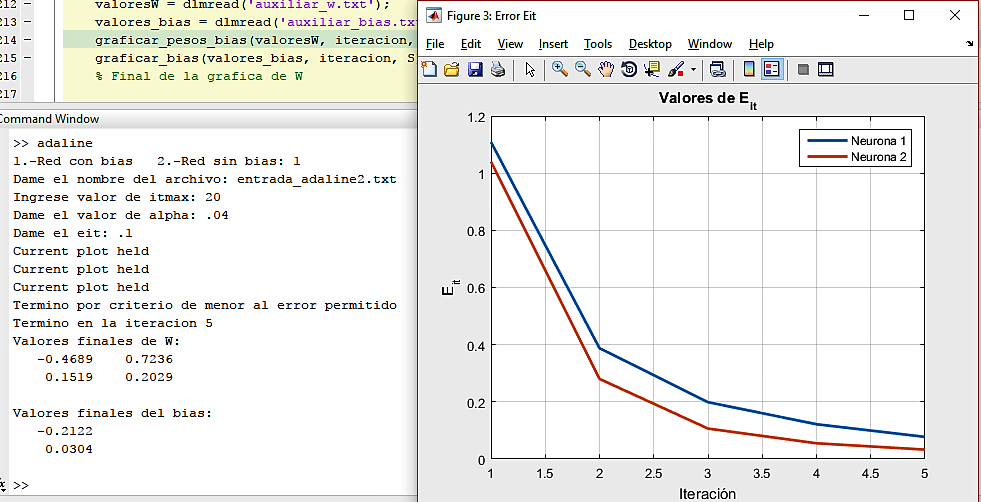
\includegraphics[width=16cm]{img/adaline2/error.png}
        \caption{Prueba 2 de ADALINE con bias.}
        \label{fig:adaline2error}
    \end{center}
\end{figure}
En esta ocasión la red convergió en la iteración 5 debido al criterio de menor al error permitido reflejado en la figura \ref{fig:adaline2error} para cada una de las neuronas que componen esta red. Los valores finales de pesos y bias se almacenaron en su correspondiente archivo de salida con los valores.
\begin{align*}
\boldsymbol{W} = \left[\begin{array}{cc}-0.4648& 0.7236\\ 0.1519& 0.2029\end{array}\right] && \boldsymbol{b} = \left[\begin{array}{c}-0.2122\\ 0.0304\end{array}\right]
\end{align*}
\begin{figure}[H]
    \begin{center}
        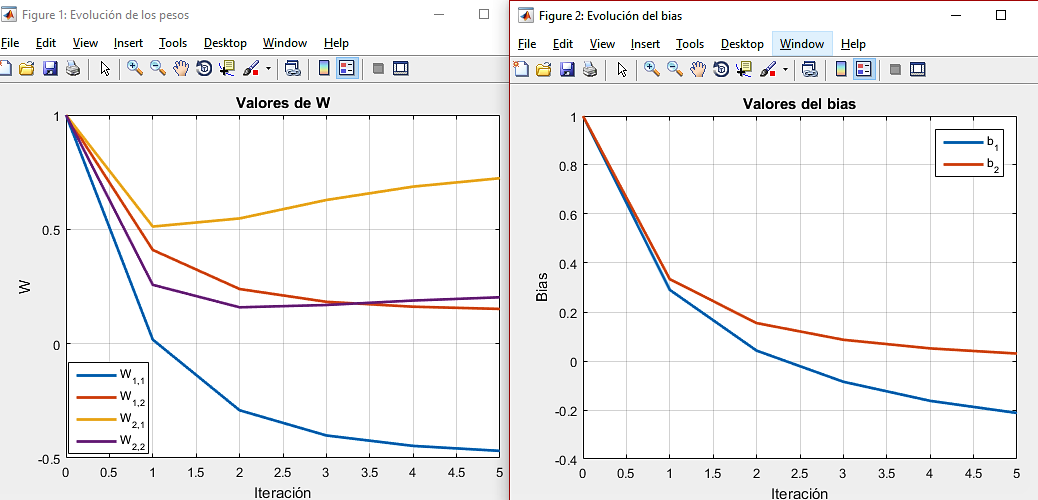
\includegraphics[width=16cm]{img/adaline2/pesosbias.png}
        \caption{Pesos y bias en esta prueba.}
        \label{fig:adaline2pesos}
    \end{center}
\end{figure}
\subsubsection{Sin bias}
\textbf{Experimento 1}. En este caso el tamaño del codificador ingresado por el usuario fue de 4, el error mínimo aceptable fue $e_{it} = 0.01$ y el valor de alpha fue $\alpha=0.02$, esto se puede observar en la figura \ref{fig:adaline3error}.
\begin{figure}[H]
    \begin{center}
        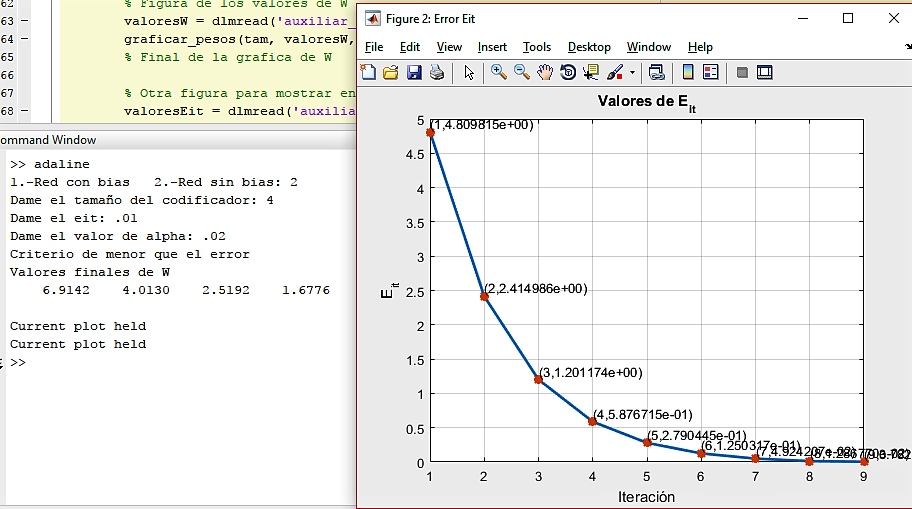
\includegraphics[width=16cm]{img/adaline3/error.png}
        \caption{Prueba 1 de ADALINE sin bias.}
        \label{fig:adaline3error}
    \end{center}
\end{figure}
La red convergió en la debido a que el error es menor al valor aceptable dando como resultado los siguientes valores de $\boldsymbol{W}$.
\[ \boldsymbol{W} = \left[\begin{array}{cccc}6.9142 & 4.0130 & 2.5192 & 1.6776\end{array}\right] \]
\begin{figure}[H]
    \begin{center}
        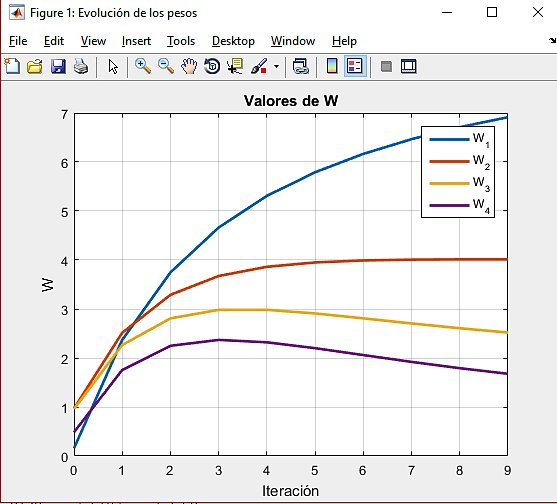
\includegraphics[width=10cm]{img/adaline3/pesosbias.png}
        \caption{Pesos de esta prueba.}
        \label{fig:adaline3pesos}
    \end{center}
\end{figure}
\textbf{Experimento 2}. En este caso el tamaño del codificador ingresado por el usuario fue de 5, el error mínimo aceptable fue $e_{it} = 0.01$ y el valor de alpha fue $\alpha=.03$, esto se puede observar en la figura \ref{fig:adaline4error}
\begin{figure}[H]
    \begin{center}
        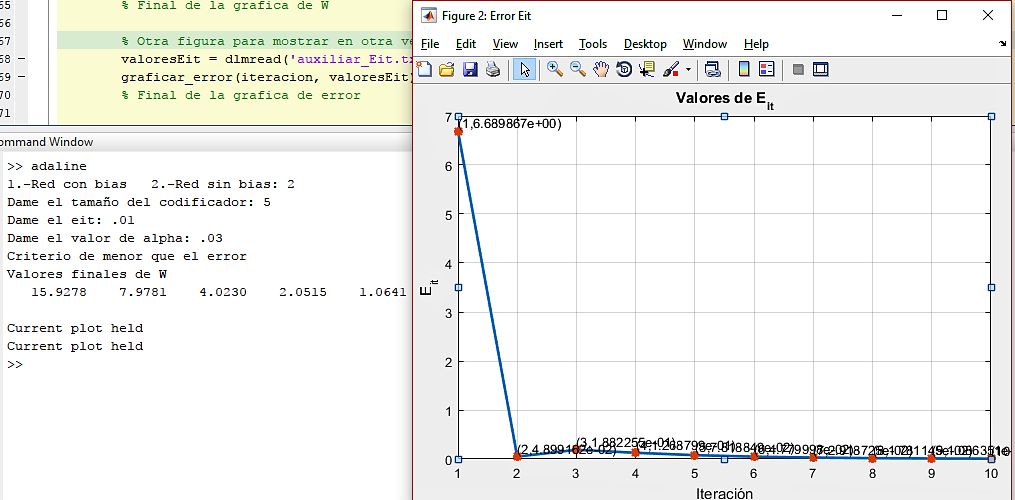
\includegraphics[width=16cm]{img/adaline4/error.png}
        \caption{Prueba 2 de ADALINE sin bias.}
        \label{fig:adaline4error}
    \end{center}
\end{figure}
La red convergió en la debido a que el error es menor al valor aceptable dando como resultado los siguientes valores de $\boldsymbol{W}$.
\[ \boldsymbol{W} = \left[\begin{array}{ccccc}15.9278 & 7.9781 & 4.023 & 2.0515 & 1.0641\end{array}\right] \]
\begin{figure}[H]
    \begin{center}
        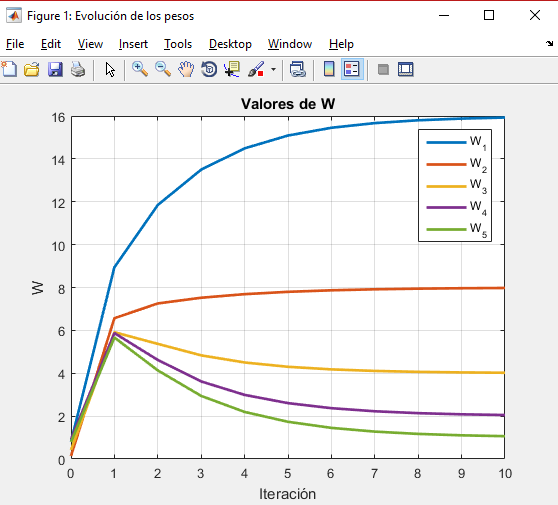
\includegraphics[width=10cm]{img/adaline4/pesosbias.png}
        \caption{Pesos de esta prueba.}
        \label{fig:adaline4pesos}
    \end{center}
\end{figure}
        